\chapter{Robot}
    The robot we simulate and use is based on the multistable joint we have seen on section \ref{sec:multistable}. In fact each leg is a multistable joint. As we have different sequences for each leg, the motion of the robot is hard to predict. We will first go through the structure of the robot before talking about the actuation of the legs. Then we will cover how the legs are articulated and how they are touching the ground. 
    
    \section{Structure}
        Let's dive into the structure of the robot, Figure \ref{fig:robot_top_view} shows a top view of the structure of the robot. Each multistable structure also consists of three blocks linked by red arms. We can recognize four multistable structures in the robot. The main frame is the yellow part of the robot, it links the bottom block of all multistable structures together, this means that the position of the four bottom blocks are static relative to each other. 
        \begin{figure}
            \centering
            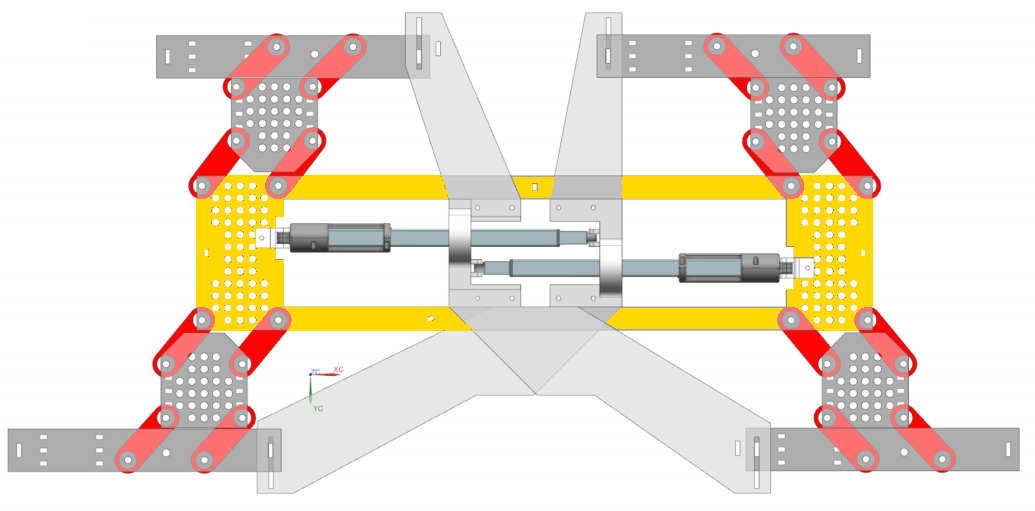
\includegraphics[width=0.8\textwidth]{images/top_view_robot.png}
            \caption{Top view of the robot. We can see four identical multistable joint that act as legs. The yellow part is the main frame. This main frame is connecting the ground block of the four multistable joint together. }
            \label{fig:robot_top_view}
        \end{figure}
    \section{Actuation}
    \section{Legs}